\documentclass{article}
\author{Isaac B Goss\\ James Hahn\\ Jonathan Dyer}
\title{Assignment 22}

\usepackage{amsmath}
\usepackage{amsthm}
\usepackage{enumitem}
\usepackage[margin=0.8in]{geometry}
\usepackage{graphicx}

% ============ USED FOR OUR FORMAT ============
\newtheorem{thm}{Claim}
\providecommand{\prob}[1]{\section*{Problem #1}}
\providecommand{\soln}{\textbf{Solution: }}
\providecommand{\image}[1]{
    \begin{center}
        \includegraphics%[width=0.95\textwidth]
            {#1}
    \end{center}
}
\providecommand{\tightlist}{
    \setlength{\itemsep}{0pt}\setlength{\parskip}{0pt}
}
\providecommand{\reducible}[2]{
  \textbf{#1} $\leq$ \textbf{#2}
}

% ============ USED FOR CODE LISTINGS ============
\usepackage{listings}
\usepackage[usenames,dvipsnames,svgnames]{xcolor}
\definecolor{javagreen}{rgb}{0.25,0.5,0.35}
\lstset{
    basicstyle   = \footnotesize,
    commentstyle = \color{javagreen},
    frame        = single,
    language     = C,
    stringstyle  = \color{orange},
    numbers      = left,
    showstringspaces=false,
    deletekeywords = {len, max, format, min},
    morekeywords = {yield, function, then, do, to},
    keywordstyle = \color{blue},
    escapeinside={(*}{*)},
    mathescape
}


\begin{document}
\maketitle
\prob{17}
I believe that in triad-free graphs... the max independent set size could be associated with the number of edges? So perhaps a line graph would give more intuition. Anyways, the problem is to show \reducible{IndependentSet}{TriadFree}. In other words, to come up with an algorithm that solves IndependentSet using TriadFree in polynomial time, so that we can show TriadFree is NP-hard. But I'm out of time, so I can only say that I think something like this would work:
\begin{lstlisting}
function IndependentSet(Graph G)
    let H = G $\times$ {v} for some new vertex v, or manipulated in some other way
    return TriadFree(H, k)
\end{lstlisting}



\prob{18}
Okay. The problem is \reducible{3-colorable}{planar 3-colorable}. We were given the graph shown below as a helper for this question. The construction of the solution is as follows:\\
\begin{itemize}
    \item After much experimentation, we discovered that no 3-coloring of the gadget is possible without coloring opposite corners ($x$ and $x'$, for example) the same color. After that you end up with one of two basic colorings, one where the center node matches all four corners, and one with two different colored pairs of corners, then the third color in the center.
    \item Simply embed the arbitrary graph in the plane and replace all necessarily crossing edges with the gadget. The new graph is clearly planar, now that every crossing has been replaced with a planar widget.
    \item Now because this crossover graph is 3-colorable if and only if opposite corners have the same color, inserting it  (or enough copies of it side by side to preserve the coloration from the outside) at any crossover with a 3-coloring \textit{will not} change the 3-colorability of the entire graph. This is because any neighboring vertex still simply sees the same color it saw before except that now the graph that edge goes to is entirely planar, along with the rest of the graph.
\end{itemize}

\begin{center}
    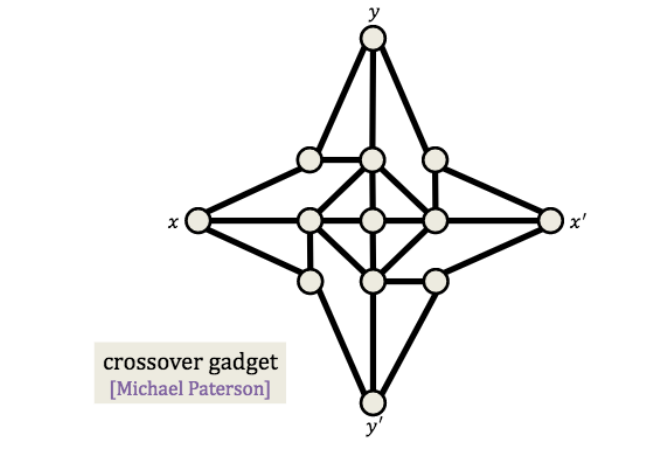
\includegraphics[width=0.5\textwidth]
        {gadget}
\end{center}

In summary, we have shown that the widget does not change the colorability of the graph, since it is always 3-colorable and from any outside perspective (i.e. that of a neighboring vertex) the graph (or multiples of it side by side) can be made to look like the vertex's old neighbor. The only difference is that now it is planar. Thus, see the following pseudocode:\\
\begin{lstlisting}
function 3colorable(Graph G)
    Construct H = G embedded in the plane arbitrarily, with the modifications made as above.
    return planar3colorable(H)
\end{lstlisting}


\prob{20}
We show that \reducible{3SAT}{DisjointPaths}. So clearly our major task is to transform a boolean CNF formuula into a graph that has some \# of vertex-disjoint paths (as described by the problem) if and only if the formula is satisfiable. The general principles are this:
\begin{itemize}
  \item Begin construction of the graph as per the hint, i.e. for each variable add a pair $s_i$ and $t_i$. Now a key point is that each of these pairs is connected by two vertex-disjoint paths of length (not including endpoints) $l$, where \textbf{$l$ is the number of clauses in the formula F}.
  \item Now we get tricky. Add \textbf{another} pair of vertices $c_i$ and $d_i$ for each clause in F, and attach them as follows. If say we're considering variable $y$ in clause $m$, and it is True in the formula, then connect the $c_m$ to an unaltered node in the False path of the corresponding pair of $s$ and $t$ for $y$. Then connect that node to $d_m$.
  \item Repeat for the remaining two variables in clause $m$, connecting the clause-vertices to the \textbf{inverse} path of the variables (so connect to True path if the var is False and vice-versa). So that at the end we have three disjoint paths from $c_m$ to $d_m$. If one of these three paths are satisfiable, then the clause is satisfiable because that means all three of its variables are not turned off (i.e. at least one of its veriable-vertices is using the path that indicates it satisfies the clause correctly). However if the clause is not satisfiable then all of the variable-paths will run through the same nodes that the clause-vertices need to get to each other, so there is no vertex-disjoint path for them. This proves our if and only if statement above.
  \item So to check for 3SAT, simply construct the graph as above (clearly polynomial-time) and then feed it into the function DisjointPaths along with a list of every variable-pair (vertices) and clause-pair (vertices). Return the result.
\end{itemize}

\end{document}
